\chapter{Physikalische Problemstellung}

Die Dynamik des betrachteten Quantensystems wird mit Hilfe der \ac{lvn} beschrieben. Sie bedient sich dem aus der Quantenstatistik bekannten Konzept des Dichteoperators für ein physikalisches System. Daher wird zunächst der Dichteoperator  eingeführt. Eine alternative Formulierung der Dynamik folgt aus einer Fourier-Transformation bezüglich der Relativkoordinate und führt auf den sog. Wigner-Formalismus. Etliche Veröffentlichungen (\cite{rossi1994monte},\cite{ringhofer},\cite{van2017efficient},\cite{schulz2016application},\cite{mains1988wigner} usw.) betreffen die Implementierung dieser sogenannten Wigner-Gleichung. Daher wird auf Unterschiede und Schwierigkeiten insbesondere hinsichtlich der Randbedingungen eingegangen. In der vorliegenden Arbeit verbleibt jedoch der Fokus auf der Ortsraumformulierung. Abschließend werden alternative Verfahren genannt und die Einordnung selbiger in den physikalischen Kontext.

\section{Dichteoperator} \index{Dichteoperator}
\label{sec:2_1}
Aus Sicht des Entwicklers elektronischer Bauelemente ist es naheliegend, nach der Elektronendichte $n(\vb{r})$ sowie der Stromdichte $j(\vb{r})$ des Systems zu fragen. Quantenmechanisch sind diese Größen Observablen, also Erwartungswerte hermitescher Operatoren bezüglich des Hilbertraums der $L^2$-Funktionen. Anschaulich ist klar, dass sich die Elektronendichte aus zwei Wahrscheinlichkeiten zusammensetzt. Erstens wird die Wahrscheinlichkeit dafür benötigt, dass ein Zustand mit Energie $\epsilon$ besetzt ist. Diese wird mit der Aufenthaltswahrscheinlichkeit, dass am Ort $\vb{x}$ überhaupt ein Teilchen vorhanden ist, multipliziert. Schließlich muss über alle Energien aufsummiert werden.

Dieser intuitive Zusammenhang wird in der Quantenstatistik mit Hilfe des sogenannten Dichteoperators beschrieben. Dazu wird der Begriff des \index{quantenmechanisches Ensemble}\emph{quantenmechanischen Ensembles} benötigt. Ein Hilbertraum $H$ sei durch eine Menge $\{\ket{k}\}$ von Zuständen mit den Eigenschaften
\begin{itemize}
  \item{i)} $\bra{k}\ket{k} = 1$
  \item{ii)} $\{\ket{k}\}$ vollständig, dh. $\ket{\Psi}=\sum_k \alpha_k\ket{k} \qquad \forall \, \ket{\Psi}\in H$ und $\ket{k}\in\{\ket{k}\}$
\end{itemize}
definiert. Da die Orthogonalität der $\ket{k}$ nicht gefordert ist, ist das System eventuell übervollständig. Ein Ensemble besteht nun aus einer großen Anzahl von Kopien des Systems, jede präpariert in einem der Zustände $\ket{k}$. Es bezeichne $w_k$ den Bruchteil der Kopien im Zustand $\ket{k}$. Per Definition ist also $w_k\geq 0$ und $\sum_k w_k = 1$.

Der Erwartungswert eines Operators ${\hat{A}:H\rightarrow H}$ lässt sich nun sinnvoll schreiben gemäß
\begin{equation*}
  \expval{\hat{A}} = \sum_k w_k \bra{k}\hat{A}\ket{k} \; .
\end{equation*}
Um diesen Erwartungswert in einer beliebigen vollständigen Orthonormalbasis $\{\ket{l}\}$ darzustellen, wird die quantenmechanische Identität $\hat{1}=\sum_l \ket{l}\bra{l}$ eingeschoben. Dann lässt sich die Information über das Ensemble elegant in einem neuen Operator $\hat{\rho}$, dem sogenannten Dichteoperator separieren. Es gilt
\begin{align}
  \expval{\hat{A}} &= \sum_l \sum_k  w_k \bra{k}\hat{A}\ket{l}\bra{l}\ket{k} \\
   &= \sum_l \bra{l}\hat{\rho} \hat{A}\ket{l} = \text{Sp}(\hat{\rho} \hat{A})
   \label{eq:expval}
\end{align}
mit
\begin{equation}
  \hat{\rho} \equiv \sum_k w_k\ket{k}\bra{k} \; .
  \label{eq:dichteoperator}
\end{equation}
Aus der Definition der $\ket{k}$ und der $w_k$ folgen drei wichtige Eigenschaften.

\begin{tabular}{l l l}
  1)  & $\hat{\rho}=\hat{\rho}^{\dagger}$ & hermitesch, \\
  2)  & $\forall \,\Psi\in H \; :\; \bra{\Psi} \hat{\rho} \ket{\Psi} \geq 0$ & positiv-semidefinit und \\
  3)  & $\text{Sp}(\hat{\rho})=1 = \expval{1}$ & normiert. \\
\end{tabular}

Der nach Gleichung \eqref{eq:dichteoperator} definierte Dichteoperator enthält vollständige Information über das System. In Vielteilchensystemen ist die Berechnung infolge begrenzter Rechenkapazität jedoch nicht möglich und es werden -- wie üblich in der Physik -- Näherungen zur Beschreibung eines Systems benötigt. Dann ist es ausreichend, das Gesamtsystem mit Hilfe des sogenannten reduzierten Dichteoperators zu beschreiben.

\section{Reduzierter Dichteoperator}\index{Reduzierter Dichteoperator}
Im Allgemeinen setzt sich der N-Teilchen-Hamiltonoperator aus Einteilchen-, Zweiteil-chen- bis zu N-Teilchen-Operatoren zusammen, die auf den jeweiligen Unterräumen des \emph{Fockraums} \index{Fockraum}
\begin{equation*}
  H = H^1 \oplus H^2 \oplus \dots \oplus H^N
\end{equation*}
agieren. Wechselwirkung zwischen Teilchen setzt naturgemäß mindestens zwei Teilchen voraus, sodass Einteilchen-Operatoren ausschließlich in $H^1$ leben. Beispiele für Einteilchenoperatoren sind kinetische Energie $\hat{T}$, Teilchenzahl $\hat{N}$ oder Stromdichte $\hat{j}$. Die potentielle Energie eines jeden Teilchens hängt jedoch im Allgemeinen von den Orten und Geschwindigkeiten aller Teilchen ab und ist daher ein $N$-Teilchen-Operator. Zur Vereinfachung dieses komplizierten Zusammenhangs wird häufig -- und so auch in dieser Arbeit -- eine \index{Mean-Field-Näherung} \emph{Mean-Field-Näherung} getroffen, wonach die wechselwirkenden Teilchen als freie Teilchen in einem externen Feld betrachtet werden. Dann enthält der Hamiltonoperator lediglich Einteilchen-Operatoren $\hat{A}_{(1)}$.

Erwartungswerte werden erneut nach Formel \eqref{eq:expval} errechnet. Es ist nun jedoch sinnvoll, die Spur in der Besetzungszahl-Basis zu notieren. Dazu werden Orts- und Impulseigenzustände (vgl. Anhang \ref{sec:A_1}) als Basis des Fockraums eingeführt gemäß
\begin{align*}
  &\ket{r_a,r_b, \dots, r_l} \equiv \ket{r_a}_1 \ket{r_b}_2 \times \dots \times \ket{r_l}_N  & &\text{Ortseigenzustände} \\
  &\ket{k_a,k_b, \dots, k_l} \equiv \ket{k_a}_1 \ket{k_b}_2 \times \dots \times \ket{k_l}_N  & &\text{Impulseigenzustände} \; ,
\end{align*}
wobei die $r_i$ bzw. $k_i$ auch den Spin beinhalten und im Falle von Fermionen wegen des Pauli-Prinzips stets $r_i\neq r_j$ bzw. $k_i \neq k_j$ für $i\neq j$ gilt. Die Notation auf der rechten Seite ist so zu verstehen, dass das nummerierte Teilchen 2 den Ort $r_b$ besetzt.

Der Übergang zur Besetzungszahl-Darstellung wird auch als \index{zweite Quantisierung} \emph{zweite Quantisierung} bezeichnet und ist beispielsweise in \cite{czycholl} erläutert. Die Basis-Zustände sind $\ket{n_1,n_2,\dots,n_{\infty}}$, wobei die $n_{\alpha}$ die Anzahl Teilchen mit Quantenzahlen $\{\alpha\}$ (zum Beispiel Spin und Impuls) bezeichnen.  Im $N$-Teilchen System ist $\sum_{\alpha} n_{\alpha} = N$. Für Fermionen gilt ferner $n_{\alpha} \in \{0,1\}$.

Da ein Einteilchenoperator nur in $H^1$ agiert, können quantenmechanische Vollständigkeitsrelationen aus eben jenem Unterraum eingeführt werden. Dann ergibt sich für den Operator $\hat{A}^N_{(1)}$
\begin{align*}
  \hat{A}^N_{(1)} = \sum_{j=1}^N \hat{A}_j = \sum_{j=1}^N \sum_{k_a} \sum_{k_b} \ket{k_a}_{j} \prescript{}{j}{\bra{k_a}}\hat{A}_j \ket{k_b}_{j} \prescript{}{j}{\bra{k_b}} \; .
\end{align*}
Für identische Teilchen kann das Matrixelement von $\hat{A}_j$ nicht von $j$ abhängen, sodass mit $\hat{A}_j \equiv \hat{A}$
\begin{equation*}
  \hat{A}^N_{(1)} = \sum_{k_a} \sum_{k_b} \bra{k_a}\hat{A} \ket{k_b} \sum_{j=1}^N \ket{k_a}_{j}  \prescript{}{j}{\bra{k_b}}
\end{equation*}
folgt. In zweiter Quantisierung $\hat{A}^N_{(1)} \rightarrow \hat{A}^{nb}_{(1)}$ ergibt sich hieraus sowohl für Bosonen als auch Fermionen \cite{modern}
\begin{align*}
  \hat{A}^{nb}_{(1)} = \sum_{k_a \, k_b} \bra{k_a}\hat{A} \ket{k_b} \hat{a}^{\dagger}_{k_a}\hat{a}_{k_b} \; ,
\end{align*}
wobei $\hat{a}_{k_a}^{(\dagger)}$ Vernichtungs- (Erzeugungs-) operator eines Teilchens mit Impuls (und Spin) $k_a$ ist. Durch Spurbildung in der Teilchenzahlbasis ergibt sich hieraus der Erwartungswert
\begin{align*}
  \expval{\hat{A}_{(1)}(t)} &= \text{Sp}(\hat{A}_{(1)}\hat{\rho}(t)) \\
  &= \sum_{\substack{\{n_{\alpha}\} \\ \sum_{\alpha} n_{\alpha} = N}} \sum_{k_a \, k_b} \bra{k_a}\hat{A} \ket{k_b}
  \bra{\{n_{\alpha}\}} \hat{a}^{\dagger}_{k_a}\hat{a}_{k_b} \hat{\rho}^{nb}(t)  \ket{\{n_{\alpha}\}} \; .
\end{align*}
Der letzte Term entspricht dem Fockraum-Matrixelement eines Einteilchen-Dichte-operators. Die Spur hierüber wird daher als \emph{reduzierte Dichtematrix}\index{Dichtematrix} (in Impulsdarstellung) $\bra{k_a}\hat{\rho}_{(1)}(t)\ket{k_b}$ bezeichnet\cite{modern}:
\begin{equation}
  \bra{k_a}{\hat{\rho}}_{(1)}(t)\ket{k_b} = \text{Sp} (\hat{a}^{\dagger}_{k_a}\hat{a}_{k_b} \hat{\rho}^{nb}(t))
  = \sum_{\substack{\{n_{\alpha}\} \\ \sum_{\alpha} n_{\alpha} = N}} \bra{\{n_{\alpha}\}} \hat{a}^{\dagger}_{k_a}\hat{a}_{k_b} \hat{\rho}^{nb}(t) \ket{\{n_{\alpha}\}} \; .
  \label{eq:redDichteOp}
\end{equation}
Dieser Operator reduziert die Suche nach Erwartungswerten im riesigen $N$-Teilchen-Hilbertraum auf ein Problem im $1$-Teilchen-Hilbertraum. Voraussetzung ist dabei, dass Zustände des $H^1$ und des $H^N$ separabel und damit nicht verschränkt sind -- was wiederum durch die \emph{Mean-Field-Näherung} gewährleistet wird.
Das Einfügen der Vollständigkeitsrelation $\int \diff r \ket{r}\bra{r} = \hat{1}$ in Gleichung \eqref{eq:redDichteOp} führt auf die Ortsdarstellung
\begin{equation}
  \expval{\hat{A}_{(1)}(t)} = \int_{D_X} \diff r_a \int_{D_X} \diff r_b \bra{r_a}\hat{A}\ket{r_b} \bra{r_b}\hat{\rho}_{(1)}(t) \ket{r_a}
  \label{eq:expval_red}
\end{equation}
mit der reduzierten Dichtematrix (in Ortsdarstellung)
\begin{equation}
\begin{aligned}
  \bra{r_b}\hat{\rho}_{(1)}(t) \ket{r_a} &= \text{Sp}(\hat{\Psi}^{\dagger}(r_a)\hat{\Psi}(r_b)\hat{\rho}^{nb}(t)) \\
   &= \sum_{\substack{\{n_{\alpha}\} \\ \sum_{\alpha} n_{\alpha} = N}} \bra{\{n_{\alpha}\}} \hat{\Psi}^{\dagger}(r_a)\hat{\Psi}(r_b)\hat{\rho}^{nb}(t) \ket{\{n_{\alpha}\}} \; ,
\end{aligned}
\label{eq:def_dichtematrix}
\end{equation}
wobei die Feldoperatoren $\hat{\Psi}(r) \equiv \sum_{k} \bra{r}\ket{k}\hat{a}_k$ Verwendung finden. Der Begriff einer Matrix folgt hierbei nicht der streng mathematischen Definition, denn die $\ket{r}$ stellen als Kontinuum eine uneigentliche Basis dar.

Um nun zum Ausgangspunkt von Kapitel \ref{sec:2_1} zurückzukehren, ist es sinnvoll, die Observable der Teilchenzahl $\hat{N}$  in Formel \eqref{eq:expval_red} einzusetzen. Für Fermionen muss wegen der Definition des Orts-Eigenzustands (vgl. Anhang \ref{sec:A_1}) $\hat{N}\ket{r}=1\ket{r}$ gelten. Dann folgt
\begin{align*}
  \expval{\hat{N}(t)} &= \int_{D_X} \diff r_a \int_{D_X} \diff r_b \, \delta(r_a-r_b) \bra{r_b}\hat{\rho}_{(1)}(t) \ket{r_a} \\
   &= \int_{D_X} \diff r \bra{r}\hat{\rho}_{(1)}(t) \ket{r} = N(t) \; ,
\end{align*}
sodass die Diagonalelemente des reduzierten Dichteoperators mit der Teilchendichte $\expval{n(r,t)}$ identifiziert werden können:
\begin{equation}
  \expval{n(r,t)} = \bra{r}\hat{\rho}_{(1)}(t) \ket{r} = \text{Sp}(\hat{\Psi}^{\dagger}(r)\hat{\Psi}(r)\hat{\rho}^{nb}(t))  \; .
  \label{eq:expval_n}
\end{equation}
Die Normierung ist für den reduzierten Dichteoperator offenbar eine andere als im Falle des vollständigen Dichteoperators, wo $\text{Sp}(\hat{\rho})=1$ gilt. Neben der Teilchendichte lässt sich des Weiteren die elektrische Stromdichte definieren. Dazu werden üblicherweise Schwerpunkt- und Relativkoordinaten $s$ und $q$ eingeführt (siehe Gleichung \eqref{eq:gedrehteKoordinaten}) und $\tilde{u}(s,q,t) = \bra{s+\frac{q}{2}}\hat{\rho}_{(1)}(t) \ket{s-\frac{q}{2}}$ gesetzt. Dann gilt \cite{lukas1}
\begin{equation}
  \expval{j(s,t)} = e\frac{\hbar}{m}\operatorname{Im}\{\left. \partial_q \tilde{u}(s,q,t)\right\rvert_{q=0}\} \; ,
  \label{eq:expval_j}
\end{equation}
was später in Kapitel \ref{sec:dynamik} noch motiviert wird.
Für die Berechnung von praktisch relevanten Erwartungswerten (Teilchenzahl, Stromdichte) ist also eine Projektion auf die Diagonale $r_a=r_b$ notwendig. Es sei bereits hier angemerkt, dass die in der Literatur auftretende \index{hydrodynamische Näherung} \emph{hydrodynamische Näherung} diese Projektion vor der Lösung der Bewegungsgleichung durchführt \cite{wiedenhaus}. Damit gehen die in der Dichtematrix enthaltenen quantenmechanischen Ortskorrelationen nicht weiter in die Rechnung ein. In der vorliegenden Arbeit wird die Projektion erst nach der Lösung der Bewegungsgleichung durchgeführt.


\section{Modellierung}
\label{sec:modellierung}
Ziel dieses Abschnittes ist es, eine \emph{\ac{rtd}} \index{resonante Tunneldiode} zu modellieren, sodass die bis hierhin entwickelte Theorie in einem praktischen Anwendungsfall zum Einsatz gebracht werden kann.

Eine \ac{rtd} nutzt den quantenmechanischen Effekt des Tunnelns aus, weshalb letztlich ein negativer differentieller Widerstand in Teilen der Strom-Spannungs-Kennlinie festzustellen ist. Aufgebaut ist die Diode aus einer Abfolge von GaAs- und AlGaAs-Schichten, wodurch zwei Potentialbarrieren entstehen, zwischen denen sich ein Quantentopf ausbildet, siehe Abbildung \ref{fig:Heterostuktur}. Letzterer ist durch die Ausprägung resonanter Energieniveaus gekennzeichnet, welche sich aus der Lösung der Schrödingergleichung ergeben (siehe auch Abschnitt \ref{sec:TFmethod}). Entspricht die Energie der injizierten Elektronen\footnote{Die Energie der injizierten Elektronen ist direkt gekoppelt mit der an die \ac{rtd} angelegten Spannung.} gerade einem der resonanten Energiewerte des Quantentopfes kommt es zum resonanten Tunneln, sodass der Stromfluss stark ansteigt. Wird die Energie weiter erhöht, bricht der Stromfluss wieder ein, da die Resonanzbedingung nicht erfüllt ist. Wie üblich wird diese Charakteristik durch thermische Energie geglättet, sodass eine Strom-Spannungs-Kennlinie wie diejenige in Abbildung \ref{fig:IVkurve} entsteht.
\begin{figure*}
    \centering
    \begin{subfigure}[b]{0.55\textwidth}
        \centering
        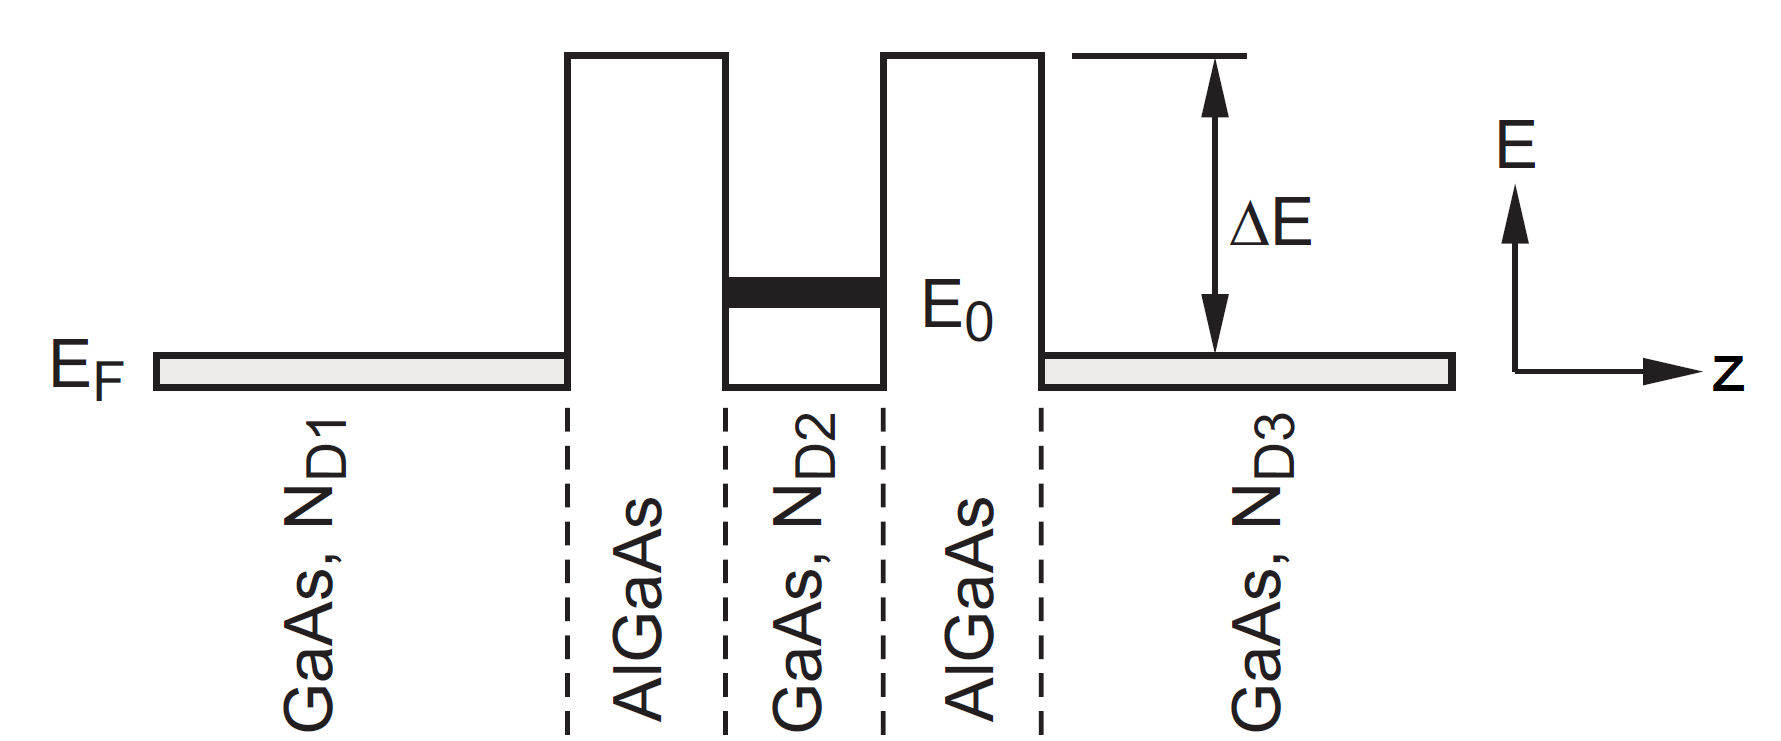
\includegraphics[width=\textwidth]{files/AlGaAs.png}
        \caption[]{{ }}
        \label{fig:Heterostuktur}
    \end{subfigure}
    \hfill
    \begin{subfigure}[b]{0.4\textwidth}
        \centering
        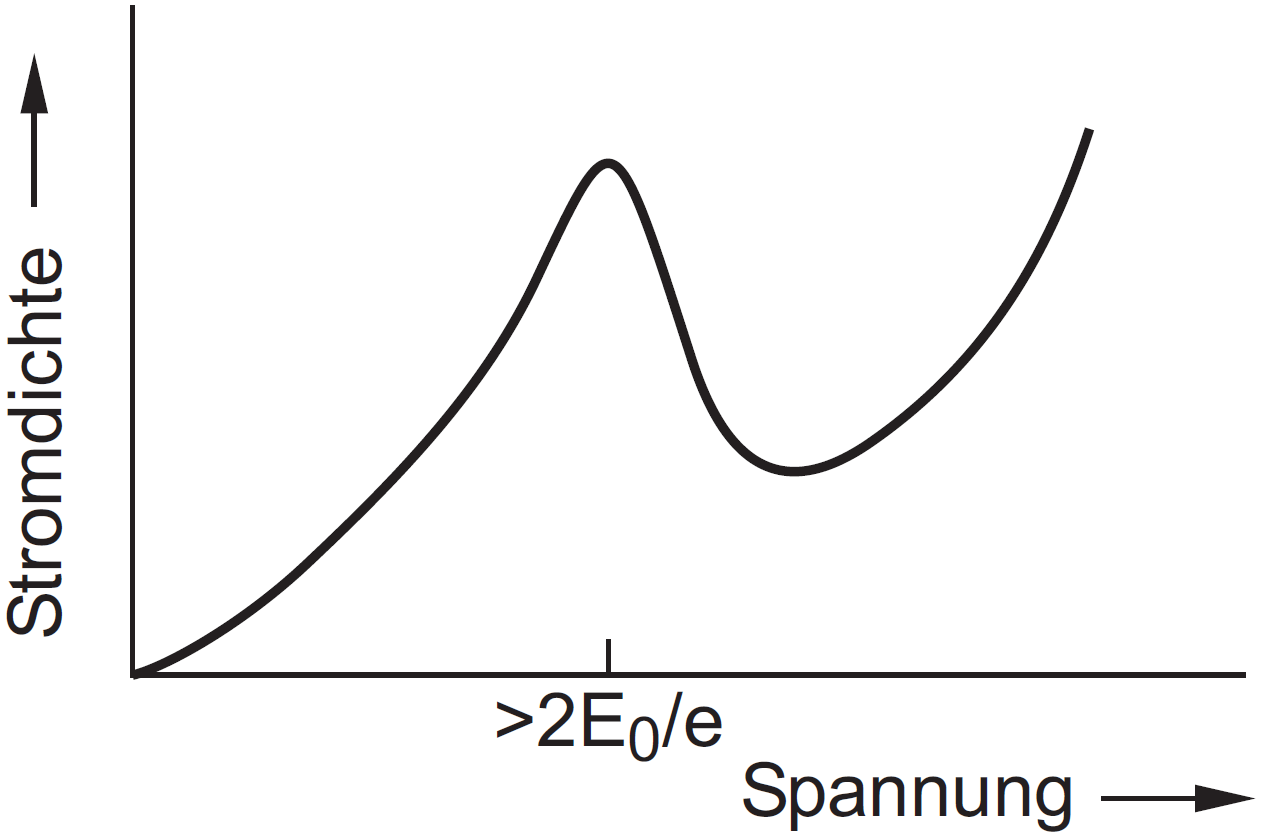
\includegraphics[width=\textwidth]{files/IVkurve.png}
        \caption[]{{ }}
        \label{fig:IVkurve}
    \end{subfigure}
    \caption[]
    {Aufbau mit Potentialverlauf (a) und Strom-Spannungs-Kennlinie einer \ac{rtd} (b), \cite{wiedenhaus}.}
    % \label{fig:Schaltungen}
\end{figure*}
Die \ac{rtd} wird im Folgenden als offenes System modelliert, durch das also Elektronen hindurchfließen können. Sie wird durch zwei Kontakte in einen Schaltkreis integriert, welche als Elektronen-Reservoire dargestellt werden. Das Modell wird nun charakterisiert durch die folgenden, vereinfachenden Anforderungen.
\begin{enumerate}[label=(\roman*)]
  \item Innerhalb der Struktur können Elektronen weder erzeugt noch vernichtet werden.
  \item Elektronen können in den Reservoiren absorbiert und erzeugt werden.
  \item Es finden keine inelastischen Streuprozesse statt, sondern ausschließlich elastische. Daher gibt es keinerlei Energiedissipation in Form von Elektron-Phonon-Wechselwirkung. Streumechanismen können im Wigner-Formalismus mit einem Kollisions-Operator beschrieben werden, näheres ist in der Literatur \cite{wiedenhaus} zu finden.
  \item Die Reservoire werden als ideale elektrische Kontakte angenommen. Sie gleichen in ihren Eigenschaften denen eines schwarzen Strahlers, siehe Kapitel \ref{sec:RB}. Innerhalb der Reservoire sind die Elektronen im thermischen Gleichgewicht mit konstanter Temperatur $T=\SI{300}{\kelvin}$ und Fermi-Niveau. Ein Stromfluss zwischen Reservoir und Quantenstruktur stellt für das Reservoir eine vernachlässigbare Störung dar \cite{frensley3}. Physikalisch ergibt sich das ideale Reservoir, wenn die Streurate in diesem sehr hoch ist bzw. die Korrelationszeit kurz ist \cite{frensley3}.
  \item Die Halbleiterschichten sind unendlich ausgedehnt, sodass die Wellenfunktionen in den transversalen Schichten die Form ebener Wellen annehmen.
  \item Der Einfluss des zugrundeliegenden Kristallgitters, durch das sich die Elektronen bewegen, wird mit Hilfe der \emph{effektiven Masse}\index{effektive Masse} beschrieben. Die effektive Masse wird in dieser Arbeit für alle Richtungen (also auch bezüglich der $z$-Richtung) als konstant angenommen, wohlwissend dass dies eine sehr grobe Näherung darstellt\footnote{Der Effekt einer nicht-konstanten effektiven Masse bezüglich $z$-Richtung wird gegenwärtig in einer anderen Arbeit am Lehrstuhl untersucht.}. Insbesondere ist durch die abrupte Änderung der Bandstruktur infolge des Heteroübergangs eine $z$-Abhängigkeit zu erwarten.
\end{enumerate}
Anforderung (iii) entspricht dem sog. kohärenten Grenzfall \cite{failure}. In diesem ist Anforderung (ii) sogar zwingend, denn sonst ließe sich ein endlicher Widerstand gemäß Abbildung \ref{fig:IVkurve} nicht erklären \cite{landauer}. Anforderung (i) muss zu einer Kontinuitätsgleichung im Inneren der Struktur führen, welche bestenfalls durch ein numerisches Schema sichergestellt wird (vgl. Abschnitt \ref{sec:IV}).

Kohärente, stationäre Zustände lassen sich mit Hilfe der \emph{single-band, effective-mass Schrödingergleichung}\index{Schrödingergleichung} \cite{frensley3}
\begin{equation}
  \begin{aligned}
    E\Psi(x) &= -\frac{\hbar^2}{2}\partial_x \frac{1}{m^*(x)}\partial_x\Psi(x) + V(x)\Psi(x)    \\
    &\approx -\frac{\hbar^2}{2m^*}\partial_x^2\Psi(x) + V(x)\Psi(x)
  \end{aligned}
  \label{eq:schroedinger}
\end{equation}
beschreiben. Hierin sind $V(x)$ das Potential und $m^*\approx 0,063m_e$\cite{GaAs} die effektive Masse von GaAs. Das Potential beinhaltet den Potentialverlauf der Heterostruktur $V_s(x,y,z)$ sowie das selbstkonsistente \emph{Hartree-Potential}\index{Hartree-Potential} $V_H(x,y,z)$ (welches das äußere Feld $-eU$ beinhaltet):
\begin{align}
  V({x}) = V_H({x}) + V_s({x}) \; .
  \label{eq:potentialgesamt}
\end{align}
Da das Hartree-Potential von der Konstellation der Elektronen abhängt und umgekehrt, wird es selbstkonsistent unter Berücksichtigung der \emph{Poisson-Gleichung}\index{Poisson-Gleichung} berechnet, wie im Anhang \ref{sec:A_4} erläutert wird.
Der durch die Materialkomposition GaAs/AlGaAs resultierende Potentialverlauf $V_s(x)$ ist in Abbildung \ref{fig:pot1} gezeigt.
\begin{figure}
  \centering
  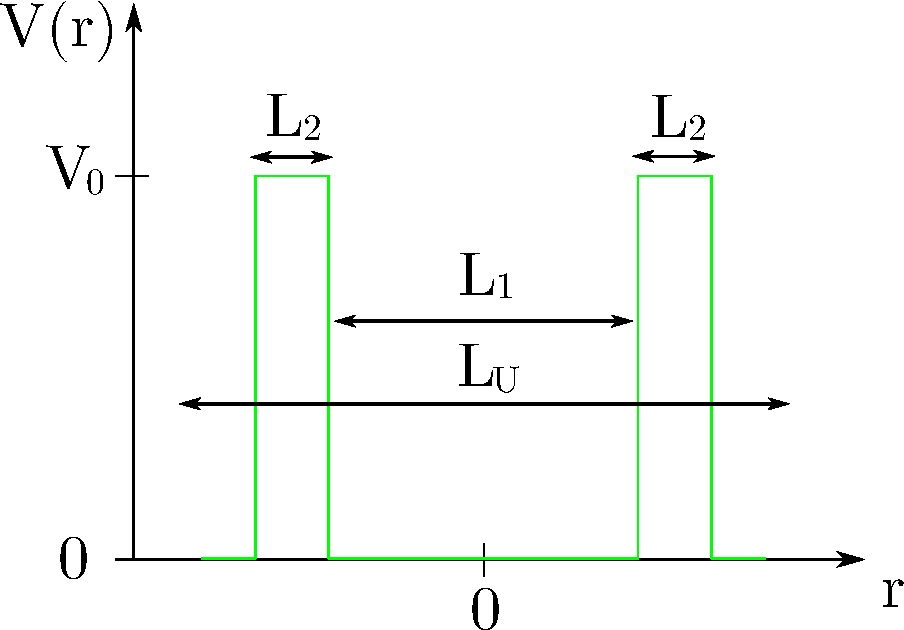
\includegraphics[width=0.7\textwidth]{files/potential.pdf}
  \caption{Potentialverlauf der \ac{rtd}.}
  \label{fig:pot1}
\end{figure}

Die quantenmechanische Beschreibung der Dynamik des Systems kann durch verschiedene Zugänge realisiert werden, siehe auch Kapitel \ref{sec:weitere_verfahren}. In der vorliegenden Arbeit wird dabei der Fokus auf die \ac{lvn} gelegt. Wie in den vorangegangenen Kapiteln erläutert, ist mit Hilfe der Dichtematrix eine Beschreibung quantenmechanischer Ensembles, also gemischter Zustände möglich. Dieser Zugang scheint für die gewählten Anforderungen unnötig verkomplizierend zu sein, jedoch ermöglicht er eine spätere Berücksichtigung von nicht-kohärenten Wechselwirkungen \cite{wiedenhaus}.


\section{Dynamik} \label{sec:dynamik}
Die Dynamik eines fermionischen Systems ergibt sich aus der \ac{lvn}. Sie lässt sich sowohl im Ortsraum, als auch im Phasenraum formulieren. Das Augenmerk dieser Arbeit richtet sich dabei auf die Ortsraumformulierung, namentlich die \ac{lvn}. Zur Vollständigkeit und zur besseren Diskussion der verschiedenen Methoden wird auch die Phasenraumformulierung vorgestellt, namentlich die Wigner-Gleichung. Das Modell für das konkrete, physikalische Problem wird dann in beiden Fällen durch die Randbedingungen beschrieben.

\subsection{Liouville-von-Neumann-Gleichung}\index{Liouville-von-Neumann-Gleichung}
Die Dynamik der reduzierten Dichtematrix \eqref{eq:def_dichtematrix} wird mit Hilfe der von-Neumann Gleichung für den Dichteoperator $\hat{\rho}(t)$
\begin{equation*}
    \partial_t \hat{\rho}(t) = - \frac{i}{\hbar}[\hat{H}(t), \hat{\rho}(t)]
\end{equation*}
hergeleitet. Es folgt nach Ausnutzen der Spurinvarianz unter zyklischem Vertauschen aus Gleichung \eqref{eq:def_dichtematrix}
\begin{align}
  \partial_t \underbrace{\bra{{r_a}}\hat{\rho}_{(1)}(t) \ket{{r_b}}}_{\equiv \rho_{(1)}({r_a},{r_b},t)} &= \text{Sp}([\hat{\Psi}^{\dagger}({r_a})\hat{\Psi}({r_b}),\hat{H}]\hat{\rho}(t)) \; .
  \label{eq:dichtematrix}
\end{align}
Die gewählte Darstellung in zweiter Quantisierung erfordert nun einen Ausdruck für den Hamiltonoperator ${\hat{H}=\hat{H}_{\text{kin}} + \hat{H}_{\text{pot}}}$. Wie bereits im vorangegangen Kapitel erwähnt, wird an dieser Stelle eine Mean-Field-Näherung getroffen, sodass sich das Potential als äußeres Potential
\begin{equation}
    \hat{H}_{\text{pot}} \approx \int_{D_X} \diff r \hat{\Psi}^{\dagger}(r)V(r)\hat{\Psi}(r)
    \label{eq:Hpot}
\end{equation}
darstellen lässt \cite{modern}. Dabei ist ${V: D_X \rightarrow \mathbb{R}}$ das äußere (gemittelte) Potential. Der kinetische Anteil ist unter der Annahme ${m(r)=\text{konst.}}$ durch
\begin{equation*}
  \hat{H}_{\text{kin}} = -\frac{\hbar^2}{2m}\int_{D_X} \diff r \hat{\Psi}^{\dagger}(r)\partial_r^2\hat{\Psi}(r)
\end{equation*}
gegeben \cite{modern}. Unter Verwendung der fermionischen Kommutator-Relationen   \cite{modern}
\begin{align*}
  [\hat{\Psi}({r_a}),\hat{\Psi}^{\dagger}({r_b})]&=\delta({r_a}-{r_b}) \\
  [\hat{\Psi}({r_a}),\hat{\Psi}({r_b})]&=0  \qquad \text{sowie}\\
  [a,bc]&=a[b,c]+b[a,c]
\end{align*}
folgt hieraus schließlich
\begin{align*}
  \partial_t \rho_{(1)}({r_a},{r_b},t) = &\frac{i}{\hbar}\left\{-\frac{\hbar^2}{2m}(\partial_{r_a}^2 - \partial_{r_b}^2) + (V({r_a},t) - V({r_b},t)) \right\} \\
                          &\times\,\text{Sp}(\hat{\Psi}^{\dagger}({r_a}) \hat{\Psi}({r_b}) \hat{\rho}(t))
\end{align*}
bzw. in der bekannteren Form mit Definition \eqref{eq:def_dichtematrix} die \ac{lvn}
\begin{equation}
  i\partial_t \rho_{(1)}({r_a},{r_b},t) = \underbrace{\left\{\frac{\hbar}{2m}(\partial_{r_a}^2 - \partial_{r_b}^2) - \frac{1}{\hbar}(V({r_a},t) - V({r_b},t)) \right\}}_{\equiv{\tilde{\mathcal{L}}({r_a},{r_b},t)}} \rho_{(1)}({r_a},{r_b},t)
  \label{eq:lvn_first}
\end{equation}
mit dem \emph{Liouvilleoperator}\index{Liouvilleoperator} $\tilde{\mathcal{L}}({r_a},{r_b},t)$. Dieselbe Gleichung ergäbe sich für den Dichteoperator, wenn der Hilbertraum von vornherein ein Einteilchenraum wäre. Mit der vorangegangen Herleitung gelingt jedoch eine allgemeinere Formulierung, die auf die entscheidende Annahme (Gleichung \eqref{eq:Hpot}) hinweist. Weiterführende Arbeiten könnten an dieser Stelle beispielsweise Zweiteilchen-Wechselwirkungen mit einbeziehen.

Zur Untersuchung der \ac{lvn} werden zwei Fälle unterschieden, worauf im Folgenden referenziert werden wird:
\begin{itemize}
  \item Der \emph{stationäre Fall}\index{stationärer Fall} mit $\partial_t \rho_{(1)}({r_a},{r_b},t) = 0$. Hier gilt ${\left[\hat{\rho} , \hat{H}\right]=0}$.
  \item der allgemeinere \emph{transiente Fall}\index{transienter Fall} $\partial_t \rho_{(1)}({r_a},{r_b},t) \neq 0$.
\end{itemize}
Wie im vorangegangen Kapitel erwähnt, wird im Folgenden freie-Teilchen-Näherung in $x$- und $y$- Richtung angenommen. Dann lässt sich mit $\lambda^2 = \hbar^2/2mk_B T$ die Dichtematrix separieren \cite{grubin1993transport} gemäß
\begin{equation}
  \rho(\vb{r},\vb{r}') = \rho({z},{z}') \exp\left( \frac{({x}-{x}')^2 + ({y}-{y}')^2}{4\lambda^2}\right) \; .
\end{equation}
Der Fokus liegt also auf einem Modell unabhängiger Elektronen in einer Dimension, sodass es genügt, die Einteilchen-Dichtematrix $\rho({z},{z}')$ zu betrachten.
Aufgrund der Struktur der Gleichung ist es sinnvoll, Schwerpunkt- und Relativkoordinaten
\begin{equation}
  \begin{aligned}
    &s \equiv \frac{{r_a}+{r_b}}{2} \qquad &q \equiv {r_a}-{r_b} \\
    \Leftrightarrow\qquad &{r_a} = s+\frac{q}{2} \qquad &{r_b} = s-\frac{q}{2}
  \end{aligned}
  \label{eq:gedrehteKoordinaten}
\end{equation}
einzuführen. Diese Koordinatendrehung erfordert es, das Potential $V(x)$ auch außerhalb von $[-L/2, L/2]$ auszuwerten. Hierfür wird
\begin{equation*}
  V(x>L/2)=V(L/2) \qquad \text{bzw.}\qquad V(x<-L/2)=V(-L/2)
\end{equation*}
angenommen. Physikalisch stellt dieser Bereich die Reservoire dar, sodass diese Annahme aus der Modellierung des Systems resultiert.
Ableitungen transformieren sich gemäß
\begin{equation*}
  \begin{aligned}
    \partial_s \partial_q  &= \partial_s \left( \frac{\partial}{\partial {r_a}} \frac{\partial {r_a}}{\partial q} + \frac{\partial}{\partial {r_b}} \frac{\partial {r_b}}{\partial q}\right) \\
     &= \left( \frac{\partial}{\partial {r_a}} \frac{\partial {r_a}}{\partial s} + \frac{\partial}{\partial {r_b}} \frac{\partial {r_b}}{\partial s}\right) \left( \frac{\partial}{\partial {r_a}} \frac{1}{2} + \frac{\partial}{\partial {r_b}} \frac{-1}{2}\right)\\
     %  &= \left( \frac{\partial}{\partial x} 1 + \frac{\partial}{\partial y} 1\right) \left( \frac{\partial}{\partial x} \frac{1}{2} + \frac{\partial}{\partial y} \frac{-1}{2}\right)\\
     % &= \frac{1}{2}\partial_x \partial_x - \frac{1}{2}\partial_x \partial_y + \frac{1}{2}\partial_y \partial_x - \frac{1}{2}\partial_y \partial_y \\
    &=  \frac{1}{2}(\partial_{r_a}^2 - \partial_{r_b}^2) \; ,
  \end{aligned}
\end{equation*}
wobei im letzten Schritt der Satz von Schwarz genutzt wird. Damit ergibt sich der transformierte Liouville Operator zu
\begin{align}
  \mathcal{L}(s,q,t) = -\frac{\hbar^2}{m} \partial_s\partial_q + \underbrace{V\left(s+\frac{q}{2},t\right) - V\left(s-\frac{q}{2},t\right)}_{\equiv \tilde{B}(s,q,t)} \; .
  \label{eq:Liouvilleoperator}
\end{align}
Hier ist nun offensichtlich, dass die Symmetrie $\mathcal{L}(s,q,t)=-\mathcal{L}(s,-q,t)$ zugrunde liegt. Der Liouvilleoperator ist also antisymmetrisch bezüglich der Relativkoordinate. Mit der Umbenennung
\begin{equation}
  \label{eq:Umbenennung}
\begin{aligned}
  \rho_{(1)}\left(s+\frac{q}{2}, s-\frac{q}{2}, t\right) &\longrightarrow \tilde{u}(s,q,t) \\
  \{ s, q, t\} &\longrightarrow \{\tilde{x}, \tilde{y}, \tilde{t}\}
\end{aligned}
\end{equation}
lautet die \ac{lvn} nun
\begin{align*}
  i\hbar\partial_{\tilde{t}} \tilde{u}(\tilde{x},\tilde{y},\tilde{t})+\frac{\hbar^2}{m}\partial_{\tilde{x}}\partial_{\tilde{y}} \tilde{u}(\tilde{x},\tilde{y},\tilde{t}) -  \tilde{B}(\tilde{x},\tilde{y},\tilde{t}) \tilde{u}(\tilde{x},\tilde{y},\tilde{t}) = 0 \; .
\end{align*}
In dieser Form lässt sich die Definition der Stromdichte (Gleichung \eqref{eq:expval_j}) motivieren. Für $\tilde{y}=0$ ist der Driftterm $\tilde{B}(\tilde{x},0,\tilde{t})$ gleich Null. Dann verbleibt mit der Definition der Teilchendichte aus Gleichung \eqref{eq:expval_n} die \emph{Kontinuitätsgleichung}\index{Kontinuitätsgleichung}
\begin{equation}
  \partial_{\tilde{t}}n(x,t) = -i\frac{\hbar}{m} \partial_{\tilde{x}} (\left. \partial_{\tilde{y}}\tilde{u}(\tilde{x},\tilde{y},\tilde{t})\right\rvert_{\tilde{y}=0}) \; .
  \label{eq:kontigl}
\end{equation}
Da $n(x,t)$ reell sein muss, muss die rechte Seite ebenfalls reell und deshalb der geklammerte Term rein imaginär sein. Mit der üblichen Kontinuitätsgleichung $\partial_t n = \partial_x j / e$ folgt hieraus genau die Definition \eqref{eq:expval_j}.

In einem abschließenden, die numerische Behandlung vorbereitenden Schritt wird die \ac{lvn} in eine einheitenlose Form gebracht, indem sie zunächst durch ein willkürliches $V_0$ geteilt wird. Energien werden dann in Einheiten von $V_0$ gemessen, und es bietet sich an, die charakteristische Größe $V_0 = \SI{0.2098}{\electronvolt}$ -- die Größe des Potentialsprungs zwischen GaAs und Al$_{0,27}$Ga$_{0,73}$As \cite{GaAs2} -- hierfür zu verwenden.
Ferner wird die folgende Skalierung eingeführt, um Zeiten und Orte ebenfalls einheitenlos zu behandeln:
\begin{equation}
  \begin{aligned}
    \left(\begin{array}{c}\tilde{x}\\\tilde{y}\end{array}\right) &= \xi \left(\begin{array}{c}x\\y\end{array}\right)   & \xi &= \sqrt{\frac{\hbar^2}{mV_0}} \\
    \tilde{t} &= \tau t   & \tau &= \frac{\hbar}{V_0} \; .
  \end{aligned}
  \label{eq:skalierung}
\end{equation}
Damit folgt
\begin{align*}
  \partial_{\tilde{t}} &= \frac{\partial}{\partial (\tau t)} = \tau^{-1} \partial_t = \frac{V_0}{\hbar} \partial_t \\
  \partial_{\tilde{x}}^2 &= \frac{\partial^2}{(\partial (\xi x))^2} = \xi^{-2} \partial_x^2 = \frac{mV_0}{\hbar^2} \partial_x^2 \; ,
\end{align*}
sodass die \ac{lvn} die Form  \index{Liouville-von-Neumann-Gleichung}
\begin{empheq}[box=\widefbox]{align}
  i \partial_t u(x,y,t)+\partial_x\partial_y u(x,y,t) - B(x,y,t) u(x,y,t) = 0
  \label{eq:lvn} \\
  \partial_x\partial_y u(x,y) = B_{\infty}(x,y) u(x,y)  \qquad \text{(stationär)}
  \label{eq:lvn_stat}
\end{empheq}
annimmt. Hierbei ist
\begin{align}
  B(x,y,t) \equiv \frac{\tilde{B}(x,y,t)}{V_0} = \frac{V\left(x+\frac{y}{2},t\right) - V\left(x-\frac{y}{2},t\right)}{V_0}
  \label{eq:driftop}
\end{align}
definiert worden.

\subsection{Wigner-Gleichung}\index{Wigner-Gleichung}\label{sec:wigner}
Ausgehend von der Einteilchen-Dichtematrix in Schwerpunkt- und Relativkoordinaten (siehe Gleichungen \eqref{eq:def_dichtematrix} und \eqref{eq:gedrehteKoordinaten}) führt eine Fourier-Transformation bezüglich der Relativkoordinate auf die sogenannte \emph{Wigner-Funktion}\index{Wigner-Funktion}
\begin{equation}
  f_{(1)}(k,s,t) \equiv \int \diff q e^{ikq}\bra{s+\frac{q}{2}}\hat{\rho}_{(1)}(t)\ket{s-\frac{q}{2}}
  \label{eq:fourier_wigner}
\end{equation}
die von Wigner \cite{wigner} 1932 eingeführt worden ist. Die inverse Abbildung ist durch
\begin{equation}
  \bra{s+\frac{q}{2}}\hat{\rho}_{(1)}(t)\ket{s-\frac{q}{2}} = \int \frac{\diff k}{2\pi}e^{-ikq} f_{(1)}(k,s,t)
  \label{eq:fourier_wigner_invers}
\end{equation}
gegeben. Im klassischen Limes ($\hbar \rightarrow 0$) geht die Wigner-Funktion in die aus der klassischen Physik bekannte Wahrscheinlichkeitsdichte im Phasenraum über. Die Position eines Teilchens wird dann mit $r$ aus Gleichung \eqref{eq:gedrehteKoordinaten} und der Impuls mit $p=\hbar k$ identifiziert.

In dieser anschaulichen Darstellung ergeben sich Erwartungswerte intuitiv durch Gewichtung der Observablen mit der Verteilungsfunktion und anschließender Integration. So lassen sich Teilchendichte und -strom gemäß
\begin{align}
  n(s,t) &= \int \frac{\diff k}{2\pi}f_{(1)}(k,s,t) \label{eq:wigner_n}\\
  j(s,t) &= \int \frac{\diff k}{2\pi}\hbar k f_{(1)}(k,s,t) \label{eq:wigner_j}
\end{align}
schreiben \cite{modern}. Die \ac{lvn} für die Wigner-Funktion lautet dann \cite{frensley2, failure}
\begin{equation}
  \partial_t f_{(1)}(k,s,t) = -\frac{\hbar k}{m}\partial_r f_{(1)}(k,s,t) - \frac{1}{\hbar} \int \frac{\diff k'}{2\pi}\mathcal{V}(k-k',s,t)f_{(1)}(k',s,t)
  \label{eq:wigner}
\end{equation}
mit dem Integralkern (auch Wignerpotential genannt)
\begin{equation*}
  \mathcal{V}(k,s,t) = 2\int_0^{\infty} \diff q \sin(k\cdot q) (V(s+\frac{q}{2},t) - V(s-\frac{q}{2},t))
\end{equation*}
und ist als Wigner-Gleichung bekannt. Sie ist das quantenmechanische Analogon zur Boltzmann-Gleichung. Das Integral auf der rechten Seite entspricht dabei einer Faltung zwischen Potentialterm und Wigner-Funktion bezüglich der Impulskoordinate $k$.



\subsection{Randbedingungen}
\label{sec:RB}
Die Dynamik des in der Einleitung skizzierten Systems muss irreversibel in der Zeit sein. Andernfalls sind instabile Lösungen in der Zeit zulässig \cite{frensley2}. Solche instabilen Lösungen lassen sich anhand des Eigenwertspektrums des Liouvilleoperators aus Gleichung \eqref{eq:lvn_first} erkennen. Es lässt sich zeigen, dass für geschlossene, konservative Systeme $\mathcal{L}$ hermitesch ist als Folge der Hermitizität des Hamiltonoperators $H$ \cite{frensley2}. Es gilt \cite{frensley2}
\begin{align*}
  H- H^{\dagger} = \frac{\hbar}{i}\int_{\partial\Omega} \vb{j}\diff\vb{s} = 0 \; .
\end{align*}
Der Nettostrom durch die Oberfläche $\partial\Omega$ ist also Null. Damit treten lediglich oszillierende Lösungen der \ac{lvn} auf. Da jedoch ein offenes System modelliert werden soll (siehe Abschnitt \ref{sec:modellierung}), muss das Ein- und Austreten von Teilchen in das System erlaubt sein, wodurch die Hermitizität von $H$ und $\mathcal{L}$ verletzt wird\cite{frensley2}.
Dadurch wird mindestens ein Eigenwert einen nicht-verschwindenden imaginären Teil bekommen. Anhand Gleichung \eqref{eq:lvn_first} ist ersichtlich, dass in der Zeit instabile Lösungen für Eigenwerte mit positivem Realteil auftreten. Falls die Randbedingungen reversibel in der Zeit sind, so sind die Realteile der Eigenwerte symmetrisch und es existieren unphysikalische, instabile Lösungen \cite{frensley2}. Ein Beispiel hierfür ist $\partial_s \rho = 0$ entlang $(r_a=\pm L/2, r_b)$ und $(r_a,r_b=\pm L/2)$. Diese Randbedingung ist insofern plausibel, da sie zu konstanter Dichte an den Rändern führt und damit den Effekt eines fixierten chemischen Potentials beschreibt. Sie führt jedoch wegen der Zeit-Umkehrbarkeit zu unphysikalisch exponentiell steigenden Lösungen \cite{frensley2}.

Die Randbedingungen müssen also irreversibel in der Zeit sein und ferner die Stabilität des Systems sicherstellen. Ein hierfür möglicherweise geeigneter Ansatz wird erstmals in \cite{frensley2} getroffen, indem die Reservoire in Analogie zu einem schwarzen Körper gesehen werden. In das Reservoir eintretende Teilchen werden vollständig absorbiert. Umgekehrt "strahlt" das Reservoir Teilchen entsprechend der thermischen Gleichgewichts-Verteilung in das System ein, siehe Abbildung \ref{fig:modell}.
\begin{figure}
  \centering
  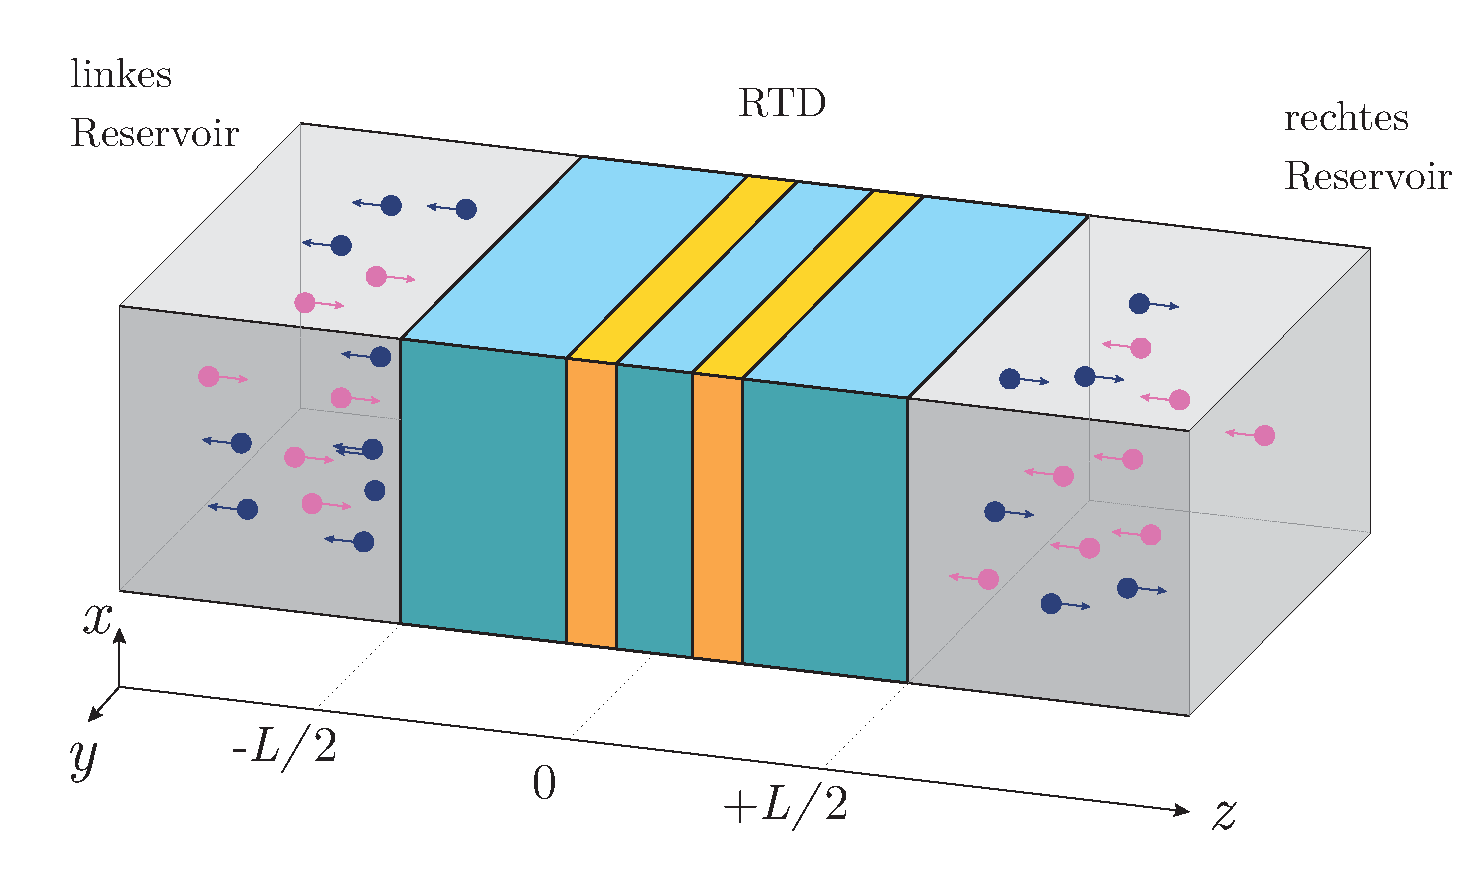
\includegraphics[width=0.7\textwidth]{files/RTD_reservoire.pdf}
  \caption{Veranschaulichung des Modells einer in einen elektrischen Schaltkreis integrierten \ac{rtd}. In den Reservoiren werden Elektronen absorbiert und emittiert. Der in rot angedeutete \emph{Inflow} wird als Randbedingung gesetzt, während der \emph{Outflow} (blau) sich durch die Transportcharakteristik der Bewegungsgleichung ergeben muss.}
  \label{fig:modell}
\end{figure}
Damit ist klar, dass Randbedingungen für Inflow-Teilchen mit positiver Geschwindigkeit am linken Rand und solche mit negativer Geschwindigkeit am rechten Rand der Domäne gesetzt sind, während für Outflow-Teilchen keine Randbedingung vorgegeben ist. Teilchen müssen also nach ihrer Geschwindigkeit unterschieden werden können.
Es ist daher ein natürliches Vorgehen, nach einer Wahrscheinlichkeitsverteilung im Phasenraum zu fragen, siehe Kapitel \ref{sec:wigner}.
Positive und negative Geschwindigkeiten lassen sich einfach durch das Vorzeichen von $k$ unterscheiden, sodass sich die Randbedingungen konkretisieren lassen:
\begin{equation}
  \begin{aligned}
    f_{(1)}(k,-L/2)|_{k>0} &= f_l({k}) \\
    f_{(1)}(k,+L/2)|_{k<0} &= f_r({k})
  \end{aligned}
  \label{eq:rb1}
\end{equation}
Die Gleichgewichts-Verteilung der Reservoire $f_{l,r}(k)$ folgt aus der Fermi-Dirac-Statistik durch Integration über die zwei freien Richtungen $k_x$ und $k_y$. Die Berechnung findet sich im Anhang \ref{sec:A_2} wieder. Es folgt
\begin{align}
  f_{l,r} (k) = \frac{m}{\pi\hbar^2\beta} \ln(1+\exp(\beta(\frac{- k^2\hbar^2}{2m} + \mu))) \; .
  \label{eq:rb2}
\end{align}
und wegen Gleichung \eqref{eq:fourier_wigner_invers} für die reduzierte Dichtematrix
\begin{equation}
  \begin{aligned}
    \rho_{(1)}(x=\pm L/2, y, t) &= \int \frac{\diff k}{2\pi} e^{iky} f(k,\pm L/2) \\
                                &= \int \frac{\diff k}{2\pi} \cos(ky) f_{\nicefrac{r}{l}} (k) \; .
  \end{aligned}
  \label{eq:rb4}
\end{equation}
Das chemische Potential $\mu$ ergibt sich dabei aus der Forderung nach Ladungsträgerneutralität im thermischen Gleichgewicht. Die Herleitung ist im Anhang \ref{sec:A_3} gezeigt.\\
Für die Ausström-Bereiche (auch \emph{Outflow} genannt) $\{ k<0, x=-L/2 \}$ und $\{ k>0, x=+L/2 \}$ trifft \eqref{eq:rb1} keine Aussage, sodass jede numerische Methode zwangsläufig ein Upwind-Schema bezüglich der $r$-Diskretisierung verwenden muss. Hierin bestätigt sich auch der Charakter der zugrundeliegenden Differentialgleichung \eqref{eq:wigner}: es wird der Transport von Elektronen beschrieben.

Eine mögliche Wahl der Randbedingungen bezüglich der Relativkoordinate für die \ac{lvn} sind Dirichlet-Randbedingungen:
\begin{equation}
  \begin{aligned}
    \rho_{(1)}(x, y=\pm L_y/2, t) = 0
  \end{aligned}
  \label{eq:rb3}
\end{equation}
Numerische Resultate zeigen für diese Wahl jedoch mitunter unphysikalische Interferenzmuster, da es an den Rändern zu Reflexion kommt \cite{lukas1}. Ein Vorschlag ist daher, eine absorbierende Schicht (\emph{\ac{cap}}\index{complex absorbing potential}) der Dicke $\delta$ einzuführen. Dabei wird der Driftterm $B(x,y,t)$ aus Gleichung \eqref{eq:lvn} um einen komplexen Teil der Größe $W_0<0$ erweitert:
\begin{equation}
  \begin{aligned}
    B(x,y,t) = \frac{V\left(x+\frac{y}{2},t\right) - V\left(x-\frac{y}{2},t\right)}{V_0} + iW(y) \qquad \text{mit} \\
  W(y)=
  \begin{cases}
  W_0 \left(y-\frac{L_y}{2}+\delta \right)^2, & \text{falls}~\frac{L_y}{2}-\delta \le y \le \frac{L_y}{2}\\
  W_0 \left(y+\frac{L_y}{2}-\delta \right)^2, & \text{falls}~-\frac{L_y}{2} \le y \le -\frac{L_y}{2}+\delta\\
  0 & \text{sonst}
  \end{cases}
  \end{aligned}
  \label{eq:cap}
\end{equation}

Die bislang beschriebenen Randbedingungen (Gleichung \eqref{eq:rb1} bzw. \eqref{eq:rb2}) sind als konventionelle oder auch U-Randbedingungen bekannt \cite{failure}. Daneben gibt es weitere Ansätze, wie absorbierende Randbedingungen \cite{arnold1994absorbing, lukas2, lukas1} und Struktur-adaptive Randbedingungen \cite{jiang2014device}. Der Grund für die Suche nach anderen Randbedingungen liegt zum Einen in der Annahme, dass an den Kontakten keinerlei Rückkopplung der Struktur  für die Elektronen zu spüren ist. Im Grenzfall einer unendlich ausgedehnten Struktur ist dies sicherlich gut begründet. Numerische Berechnungen erfordern jedoch stets ein endliches Rechengebiet. Ferner sind physikalische Strukturen immer endlich und durch echte Volumina gekennzeichnet. Korrekte Randbedingungen setzen demnach das Wissen über den Zustand des Systems voraus \cite{ringhofer}.
Kriman et al. \cite{kriman1987scattering} haben gezeigt, dass Quanteneffekte über einige thermische Wellenlängen abklingen. In \cite{ringhofer} wird für eine typische GaAs Struktur bei $\SI{300}{\kelvin}$ eine Abklinglänge von ca. $\SI{100}{\nano\meter}$ angegeben.

Zweitens ist nicht geklärt, wie Randbedingungen bezüglich der Relativkoordinate in der Ortsraumformulierung zu setzen sind. Die meisten Arbeiten beschäftigen sich mit der Wigner-Gleichung \eqref{eq:wigner}. Im Gegensatz zur \ac{lvn} taucht keine zweite Ableitung auf, sodass bezüglich der $k$-Richtung keine Randbedingungen benötigt werden \cite{frensley2}.
Es ist also insbesondere die Thematik der Randbedingungen, worin sich die beiden Formalismen unterscheiden, wodurch also die Äquivalenz von Wigner- und Schrödingerformalismus aufgehoben wird \cite{li2014stationary}.

Die Arbeit von Rosati et al. \cite{failure} weist darauf hin, dass die von Frensley eingeführten Inflow-Randbedingungen zwar semiklassisch zulässig sind, jedoch ihre Verwendung für quantenmechanische Probleme im Allgemeinen nicht gerechtfertigt ist. Dies lässt sich auf die Tatsache zurückführen, dass die semiklassische Boltzmann-Gleichung lokal in $k$ ist, während das quantenmechanische Pendant -- die Wigner-Gleichung -- nicht-lokal in $k$ ist, denn durch die Faltung in Gleichung \eqref{eq:wigner} entsteht eine Kopplung zwischen $k$ und allen anderen $k$-Punkten.
Die Autoren  des Artikels gehen unter Bezug auf den Wigner-Formalismus zwei grundlegenden Fragen nach.
\begin{enumerate}[label=(\roman*)]
  \item Ist die Lösung der Differentialgleichung mit den gegebenen Randbedingungen physikalisch akzeptabel? Für die Dichtematrix bedeutet dies insbesondere, dass sie zu positiver Ladungsträgerdichte führen muss.
  \item Ist die Lösung eindeutig?
\end{enumerate}
Während die semiklassische Boltzmann-Gleichung aufgrund ihres lokalen Charakters eine eindeutige Lösung besitzt, ist dies für die Wigner-Gleichung nicht der Fall. Abbildung \ref{fig:nonuniqueness} zeigt exemplarisch verschiedene stationäre Lösungen für den analytisch lösbaren Fall eines $\delta$-Potentials.
\begin{figure}
  \centering
  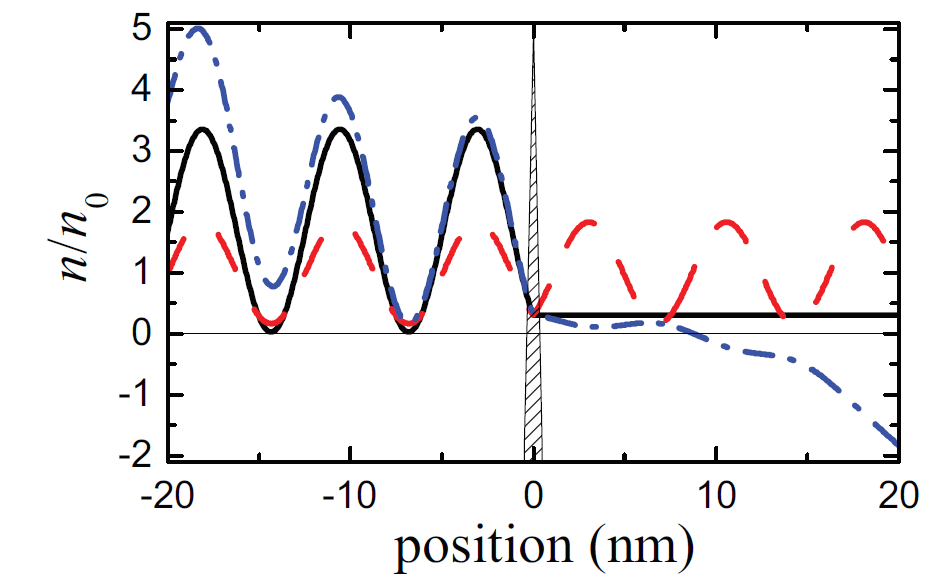
\includegraphics[width=0.7\textwidth]{files/nonuniqueness.png}
  \caption{Nicht-Eindeutigkeit der Wigner-Gleichung für den Fall eines $\delta$-Potentials, \cite{failure}.}
  \label{fig:nonuniqueness}
\end{figure}
Die Lösungen ergeben sich dabei aus einer Linearkombination von generischen Vorwärts- und Rückwärts-Streuzuständen, resultierend aus der Zeitumkehr-Symmetrie der stationären Gleichung. Letztere äußert sich auch in der energetischen Zweifach-Entartung der Streuzustände. Eine kurze Rechnung zeigt nämlich, dass wegen der Antisymmetrie des Wignerpotentials sowie der Gruppengeschwindigkeit $v(k) = \hbar k/m$ bezüglich $k$ für jede Lösung $f_{(1)}(k,r)$ auch ${g_{(1)}(k,r) = f_{(1)}(-k,r)}$ Lösung der stationären Wigner-Gleichung ist. Die Randbedingungen geben zwar eine eindeutige Überlagerung, also einen eindeutigen Satz von Koeffizienten $\{a(k)\}$  aller Vorwärts-Streuzustände vor. Da jedoch die Rückwärts-Streuzustände im Allgemeinen linear unabhängig von den Vorwärts-Streuzuständen sind, ist mit denselben Randbedingungen ein doppelt so großer Satz $\{a(k),b(k)\}$ von Koeffizienten zu finden. Das zuvor eindeutige Problem ist in diesem Fall nicht mehr eindeutig lösbar. In der Abbildung sind drei verschiedene Verhältnisse $c=b(k)/a(k)$ zu sehen, darunter auch eine unphysikalische Lösung mit negativer Teilchendichte. Für ausschließlich lokalisierte Zustände, wie sie bei parabolischen oder Quantentopf-Potentialen (mit unendlich großen Barrieren) entstehen, lässt sich jedoch nicht zwischen Vorwärts- und Rückwärts-Streuzuständen unterscheiden sodass eine eindeutige Lösung der Wigner-Gleichung zu erwarten ist \cite{failure}.

Es ist anzumerken, dass dieselbe Argumentation  im allgemeinen Fall der transienten Wigner-Gleichung nicht funktioniert. Dieses Anfangsproblem ist hingegen eindeutig lösbar, wie die Ausarbeitung in \cite{dimov2015boundary} zeigt. Es ist daher zu schlussfolgern, dass die Vorgabe einer Anfangsbedingung zu einer spezifischen Lösung aus der unendlichen Menge möglicher stationärer Lösungen führt, und somit die Anfangsbedingung das entscheidende Kriterium für eine physikalisch akzeptable Problemstellung darstellt. Die Wigner-Gleichung erhält in Bezug auf den Anfangszustand darüber hinaus sogar die Eigenschaft (i) \cite{dimov2015boundary}.

Die vorangegangenen Gedanken lassen sich auf die \ac{lvn} übertragen. Insbesondere die Inversionssymmetrie der stationären Lösung soll im Folgenden gezeigt werden. Es sei $u(x,y)$ Lösung der stationären \ac{lvn} \eqref{eq:lvn_stat}. Dann ist wegen $B(x,y)=-B(x,-y)$ auch $v(x,y)\equiv u(x,-y)$ Lösung, denn
\begin{align*}
  & &-\partial_x \partial_{\xi} u(x,{\xi}) &= - B_{\infty}(x,{\xi})u(x,{\xi}) \\
  &\Leftrightarrow &\partial_x \partial_y u(x,-y) &= - B_{\infty}(x,-y)u(x,-y) \\
  & & &=  B_{\infty}(x,y)u(x,-y) \\
  &\Leftrightarrow &\partial_x \partial_y v(x,y) &=  B_{\infty}(x,y)v(x,y) \; .
\end{align*}

Abschließend ist zu sagen, dass die gesamte Thematik der Randbedingungen Gegenstand aktueller Forschung ist \cite{jiang2011accuracy} und die hier gezeigten Aspekte nur einen kleinen Bruchteil der Komplexität darstellen. So verkompliziert sich die gesamte Fragestellung beispielsweise dramatisch, wenn die Mean-Field-Näherung fallengelassen wird und auch nicht-kohärente Effekte berücksichtigt werden. Eine gute Übersicht bieten die Arbeiten von Rossi \cite{buchRossi} und Frensley \cite{frensley}. Für die konkrete numerische Implementierung wird auf die vergleichsweise simplen Resultate \eqref{eq:rb1}, \eqref{eq:rb3} sowie Gleichung \eqref{eq:cap} zurückgegriffen.

\section{Weitere Verfahren}\label{sec:weitere_verfahren}
Neben dem hier verwendeten Dichtematrix- bzw. Wigner-Formalismus gibt es einige weitere Möglichkeiten, die stationäre Lösung sowie die Zeitentwicklung für verschiedene Fälle (Gleichgewicht, Nahe-Gleichgewicht und Fern-vom-Gleichgewicht) zu berechnen. Der Artikel \cite{frensley3} bietet einen guten Überblick über die wichtigsten Verfahren. Eine vollständige Theorie gelingt demnach lediglich mit dem \emph{\ac{negf} approach}\index{nonequilibrium Green's function}, welcher auf den Keldysh-Formalismus zurückzuführen ist. Die Grundidee dabei ist eine diagrammatische Störungstheorie, welche sowohl Vorwärts- als auch Rückwärts-Konturen mit Hilfe von vier Greens-Funktionen berücksichtigt. Die konkrete, vollständige Berechnung mit Hilfe der \ac{negf} gestaltet sich anscheinend schwierig. Die Veröffentlichungen konzentrieren sich zumeist auf Hybridverfahren (z.B. \cite{memory2, negf-dft}) oder Spezialfälle wie dem stationären Fall \cite{negf_datta}.
An dieser Stelle soll lediglich festgehalten werden, dass in einer hierarchischen Betrachtungsweise der Dichtematrix-Formalismus weniger Information enthält, denn die Dichtematrix folgt aus einer Integration
\begin{equation*}
  \rho(x,y,t) = \int \frac{\diff E}{2\pi}G^{<}(x,y;E,t) \; .
\end{equation*}
Deshalb ist die \ac{lvn} lediglich dazu in der Lage, ein Markov-Verhalten zu beschreiben, wo also externe Wechselwirkung ausschließlich instantan in der Zeit erfolgt \cite{frensley3}. Als Beispiel für das Versagen des Dichtematrix-Formalismus wird die resonante Absorption oder Emission eines Phonons genannt, für die die Schwingungsperiode des Phonons die Mindestdauer der Wechselwirkung vorgibt. Ein Verfahren, dessen Verteilungsfunktion nicht von allen drei Variablen -- Ort, Impuls und Geschwindigkeit -- abhängt, wird für die entsprechend fehlende Variable eine Erhaltungsgleichung nicht berücksichtigen \cite{frensley3}. Im Falle der \ac{lvn} ist dies die Energieerhaltung, was jedoch mit der Modellierung des Systems vereinbar und sogar notwendig ist, siehe Kapitel \ref{sec:modellierung}. Es gibt Ansätze, diesem Umstand mit Hilfe eines "Gedächtnis-Terms" beizukommen \cite{memory1, memory2}.

Ein Verfahren, welches den Spezialfall des stationären Problems im Gleichgewichtsfall beschreiben kann, wird im folgenden Kapitel \ref{sec:TFmethod} erläutert werden, denn es dient für die numerischen Tests in Kapitel \ref{sec:rates} als Referenz. Eine numerische Beschreibung, welche nicht analytisch, sondern mit der Finiten Elemente Methode die Schrödingergleichung löst und dabei die Offenheit des Systems berücksichtigt, wurde von Lent und Kirkner \cite{qtbm} erarbeitet und ist als \ac{qtbm} bekannt.

\subsection{Transfermatrix Methode}\index{Transfermatrix Method}
\label{sec:TFmethod}
Die Berechnung von reinen Zuständen ist unter Annahme der Stetigkeit von $\Psi(x)$ und $\Psi'(x)$ für den Gleichgewichtsfall anhand Gleichung \eqref{eq:schroedinger} analytisch möglich. Dazu wird als Lösung eine Linearkombination von rechts- und linkslaufender ebener Welle angenommen:
\begin{equation*}
  \begin{aligned}
    \Psi_k(z)=
    \begin{cases}
    a_{l,1}e^{ikz} + a_{l,2}e^{-ikz}              & z\in[-L/2,z_1] \\
    c_{l,1}e^{i\kappa z} + c_{l,2}e^{-i\kappa z}  & z\in[z_1, z_2] \\
    a_{m,1}e^{ikz} + a_{m,2}e^{-ikz}              & z\in[z_2,z_3] \\
    c_{r,1}e^{i\kappa z} + c_{r,2}e^{-i\kappa z}  & z\in[z_3, z_4] \\
    a_{l,1}e^{ikz} + a_{l,2}e^{-ikz}              & z\in[z_4, +L/2] \\
    \end{cases}
  \end{aligned}
\end{equation*}
Hierbei ist $k=\sqrt{2mE/\hbar^2}$ und $\kappa=\sqrt{2m(V_0-E)/\hbar^2}$.
Für das konkrete Problem einer \ac{rtd} zeigt Abbildung \ref{fig:tf1} die Zuordnung der Koeffizienten und Koordinaten.
\begin{figure}
  \centering
  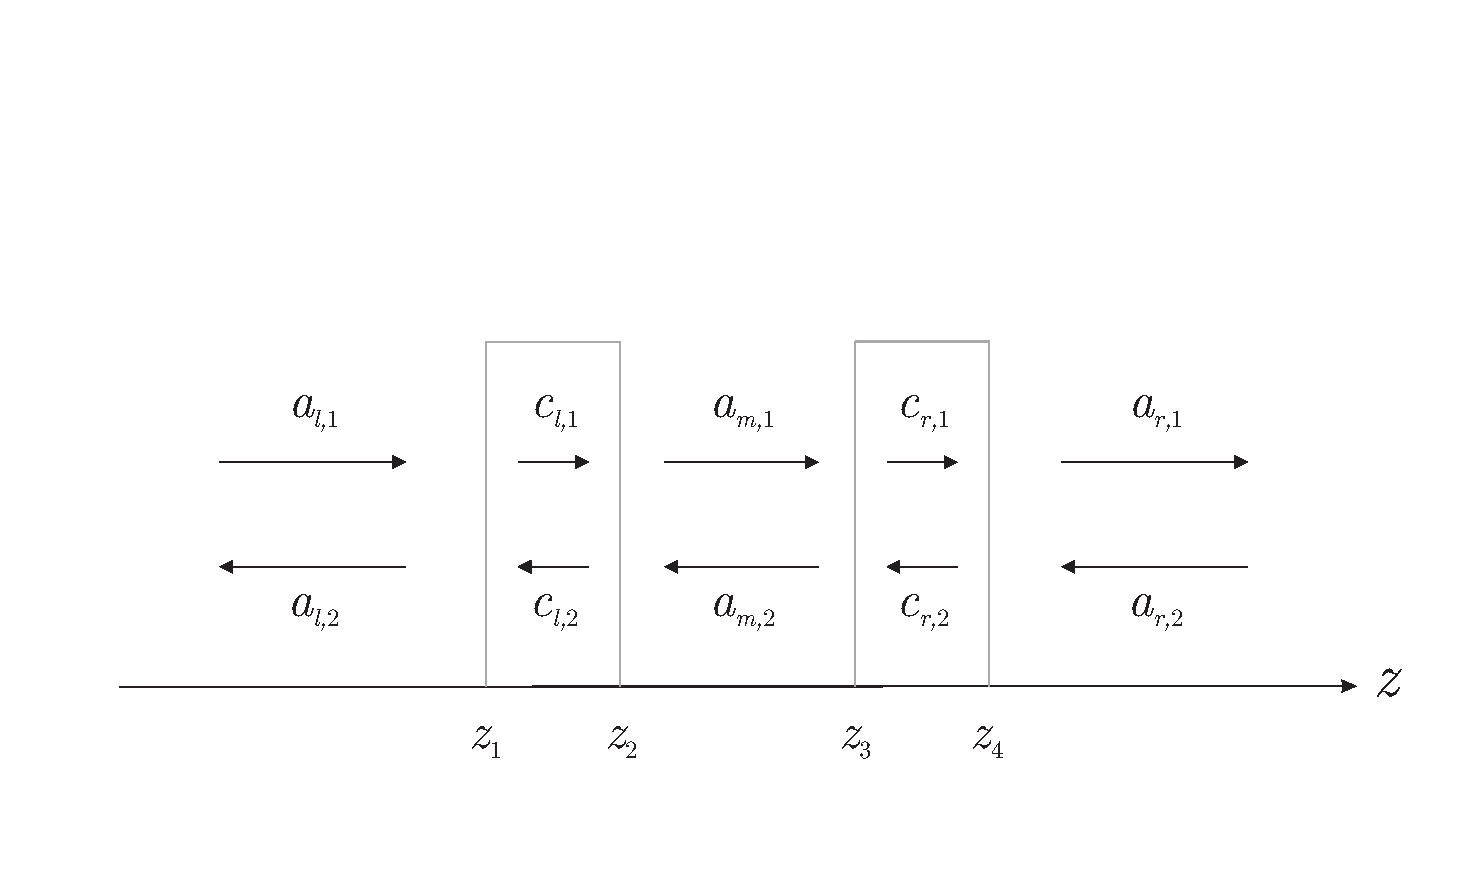
\includegraphics[width=0.7\textwidth]{files/TF_variables.pdf}
  \caption{Koeffizienten für hin- und rücklaufende Wellen mit angedeutetem Potentialverlauf der \ac{rtd}.}
  \label{fig:tf1}
\end{figure}
Mit Hilfe der erwähnten Stetigkeitsbedingung lassen sich acht der zehn Koeffizienten eliminieren, sodass sich mit $\vec{a}\equiv(a_1, a_2)^T$ letztlich
\begin{equation*}
  \vec{a_r} = \underline{\underline{S}} \vec{a_l}
\end{equation*}
schreiben lässt. Dabei hängt die Transfermatrix $\underline{\underline{S}}$ von der Energie $E(k)$ ab und ihre Existenz ist für $k\neq 0$ sichergestellt.
Der Fall $k=0$ stellt gebundene Zustände dar, welche mit dieser Methode nicht erfasst werden können. Die verbliebenen zwei Freiheitsgrade repräsentieren die Notwendigkeit der Randbedingungen. Nun ist es wichtig, die Anforderungen aus Kapitel \ref{sec:modellierung} korrekt zu berücksichtigen. Eingespeiste Elektronen kommen entweder von links, oder von rechts. Sie werden dabei vollständig dekorreliert angesehen, daher muss ${a_{r,2}=1-a_{l,1}}$ und ${a_{l,1}\in\{0,1\}}$ gelten.

Um nun aus der Energie-abhängigen Wellenfunktion die Dichtematrix zu errechnen, wird Gleichung \eqref{eq:dichteoperator} verwendet:
\begin{equation*}
  \rho(x,y) = \sum_k \omega_k \underbrace{\bra{x}\ket{k}}_{\equiv\Psi_k(x)}\bra{k}\ket{y}
\end{equation*}
Der Übergang vom Ein- zum $N$-Teilchen System gelingt, indem nun die Normierung $\sum_k \omega_k = 1$ fallen gelassen und
\begin{equation*}
  \sum_k \omega_k  \Psi_k(x) \Psi_k^{\dagger}(y) \rightarrow \int \diff k \frac{m}{\pi\hbar^2\beta} \ln(1+\exp(\beta(\frac{- k^2\hbar^2}{2m} + \mu))) \Psi_k(x) \Psi_k^{\dagger}(y)
\end{equation*}
angesetzt wird, vergleiche hierzu auch die Überlegung im Anhang \ref{sec:A_2} und in Kapitel 7 des Buches von Datta \cite{datta}. Dazu wird die Wellenfunktion gemäß den obigen Überlegungen als gleichgewichtete Summe von linksseitig (${a_{l,1}=1}$) und rechtsseitig (${a_{r,2}=1}$) eingespeistem Elektron zu
\begin{equation*}
  \Psi_k(x) = \frac{1}{\sqrt{2}}(\Psi_k^r(x) + \Psi_k^l(x))
\end{equation*}
gewählt. Das vorgestellte Verfahren ist als \ac{tf} bekannt.
